\chapter{互联网服务基础之DNS\&SSH}
\begin{center}{\textcolor[RGB]{255, 0, 0}{\faHeart}~温柔正确的人总是是难以生存,因为这个世界既不温柔,也不正确。~\textcolor[RGB]{255, 0, 0}{\faHeart}}
\end{center}
\begin{center}
	\pgfornament[width=0.36\linewidth,color=lsp]{88}
\end{center}
\section{基本网络概念解释}
\subsection{局域网|广域网|城域网}
计算机网络,按照地理位置可以划分为三类:局域网、城域网、广域网。
\begin{itemize}
	\item 局域网,LAN(Local Area Network),在较小的地理区域内建立的计算机网络。
	
	例如实验室建一个网络,内部的电脑互联起来,就是一个局域网;
	一家公司建一个网络,也是局域网,家里装个路由器,也是一个局域网。
	\item 城域网,MAN(Metropolitan Area Network),若干个局域网互相连接而成,适合于大都市的较大规模的计算机网络。
	\item 广域网,WAN(Wide Area Network),涉及几个城市、一个国家、各个国家一个的计算机网络。
	
\end{itemize}
局域网,LAN(Local Area Network),在较小的地理区域内建立的计算机网络。
\subsection{什么是IP地址}
IP地址(Internet Protocol Address)是指互联网协议地址,又译为网际协议地址。

IP地址是IP协议提供的一种统一的地址格式,它为互联网上的每一个网络和每一台主机分配一个逻辑地址,以此来屏蔽物理地址的差异。

\begin{ascolorbox5}{IP地址类型}
	\begin{ascboxB}{公网IP:}
Public IP : 公共 IP ,经由 INTERNIC 所统一规划的 IP,有这种 IP 才可以连上 Internet ;
\end{ascboxB}
	\begin{ascboxB}{私有IP:}
Private IP : 私有 IP 或保留 IP,不能直接连上 Internet 的 IP , 主要用于局域网络内的主机联机规划。	
\end{ascboxB}
\end{ascolorbox5}
\begin{ascolorbox5}{IP地址划分}
	\begin{ascboxB}{ip地址主要分为四类}
\begin{itemize}
	\item A类,ip范围0.0.0.0~126.255.255.255,A类地址主要分配给超大型网络环境的公司,例如苹果公司。
	\item B 类,ip范围128.0.0.0~191.255.255.255,主要分配给有大规模局域网数量的公司
	\item C 类,ip范围192.0.0.0~223.255.255.255,主要分配给如校园网等小型局域网
	\item D类和E类地址比较特殊,D类属于广播地址,E类属于保留地址
\end{itemize}
	\end{ascboxB}
\end{ascolorbox5}

\section{域名系统(DNS)}
虽然因特网上的节点都可以用IP地址唯一标识,并且可以通过IP地址被访问,但即使是将32位的二进制IP地址写成4个0$\sim$255的十位数形式,也依然太长、太难记。因此,人们发明了域名(Domain Name),域名可将一个IP地址关联到一组有意义的字符上去。用户访问一个网站的时候,既可以输入该网站的IP地址,也可以输入其域名,对访问而言,两者是等价的。例如:微软公司的Web服务器的IP地址是207.46.230.229,其对应的域名是www.microsoft.com,不管用户在浏览器中输入的是207.46.230.229还是www.microsoft.com,都可以访问其Web网站。
\subsection{DNS 域名解析服务}

域名系统(英文:Domain Name System,缩写:DNS)是互联网的一项服务。它作为将域名和IP地址相互映射的一个分布式数据库,能够使人更方便地访问互联网。DNS使用UDP端口53。当前,对于每一级域名长度的限制是63个字符,域名总长度则不能超过253个字符。。就像拜访朋友要先知道别人家怎么走一样,Internet上当一台主机要访问另外一台主机时,必须首先获知其地址,TCP/IP中的IP地址是由四段以“.”分开的数字组成(此处以IPv4的地址为例,IPv6的地址同理),记起来总是不如名字那么方便,所以,就采用了域名系统来管理名字和IP的对应关系。

相较于由数字构成的IP 地址,域名更容易被理解和记忆,所以我们通常更习惯通过域名
的方式来访问网络中的资源。但是,网络中的计算机之间只能基于IP 地址来相互识别对方的
身份,而且要想在互联网中传输数据,也必须基于外网的IP 地址来完成。

为了降低用户访问网络资源的门槛,DNS(Domain Name System,域名系统)技术应运
而生。这是一项用于管理和解析域名与IP 地址对应关系的技术,简单来说,就是能够接受用
户输入的域名或IP 地址,然后自动查找与之匹配(或者说具有映射关系)的IP 地址或域名,
即将域名解析为IP 地址(正向解析),或将IP 地址解析为域名(反向解析)。这样一来,我
们只需要在浏览器中输入域名就能打开想要访问的网站了。DNS 域名解析技术的正向解析也是我们最常使用的一种工作模式。鉴于互联网中的域名和IP 地址对应关系数据库太过庞大,DNS 域名解析服务采用了类
似目录树的层次结构来记录域名与IP 地址之间的对应关系,从而形成了一个分布式的数据库
系统

域名后缀一般分为国际域名和国内域名。原则上来讲,域名后缀都有严格的定义,但在
实际使用时可以不必严格遵守。目前最常见的域名后缀有.com(商业组织)、.org(非营利组
织)、.gov(政府部门)、.net(网络服务商)、.edu(教研机构)、.pub(公共大众)、.cn(中国
国家顶级域名)等。

DNS 技术作为互联网基础设施中重要的一环,为了为网
民提供不间断、稳定且快速的域名查询服务,保证互联网的正常运转,提供了下面三种类型
的服务器。

\begin{itemize}
	\item \md{主服务器}:在特定区域内具有唯一性,负责维护该区域内的域名与IP 地址之间的对
	应关系。
	\item \md{从服务器}:从主服务器中获得域名与IP 地址的对应关系并进行维护,以防主服务器
	宕机等情况。
	\item \md{缓存服务器}:通过向其他域名解析服务器查询获得域名与IP 地址的对应关系,并
	将经常查询的域名信息保存到服务器本地,以此来提高重复查询时的效率。
\end{itemize}

\subsection{DNS解析过程}
DNS 域名解析服务采用分布式的数据结构来存放海量的“区域数据”信息,在执行用户
发起的域名查询请求时,具有\md{递归查询}和\md{迭代查询}两种方式。所谓递归查询,是指DNS 服务
器在收到用户发起的请求时,必须向用户返回一个准确的查询结果。如果DNS 服务器本地没
有存储与之对应的信息,则该服务器需要询问其他服务器,并将返回的查询结果提交给用户。

而迭代查询则是指,DNS 服务器在收到用户发起的请求时,并不直接回复查询结果,而是告
诉另一台DNS 服务器的地址,用户再向这台DNS 服务器提交请求,这样依次反复,直到返
回查询结果。
\begin{figure}[H]
	\centering
	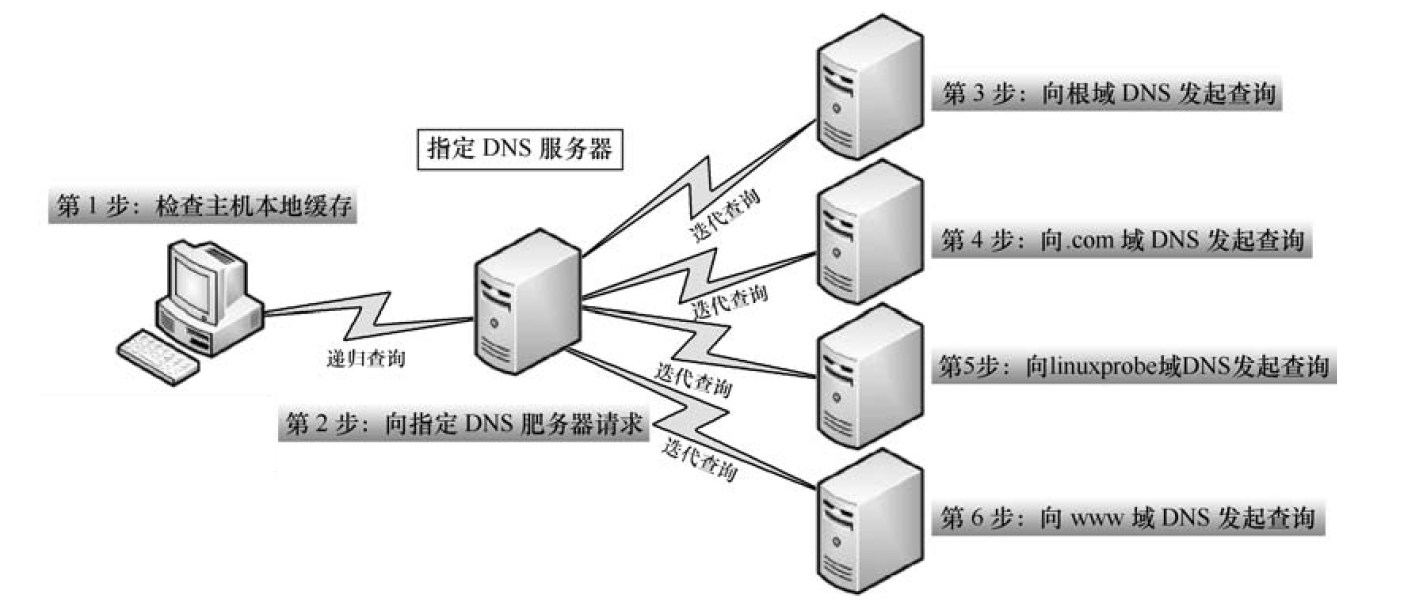
\includegraphics[width=0.8\linewidth]{image/DNS}
\end{figure}
当用户向网络指定的DNS 服务器发起一个域名请求时,通常情况下会有本地由此DNS
服务器向上级的DNS 服务器发送迭代查询请求;如果该DNS 服务器没有要查询的信息,则
会进一步向上级DNS 服务器发送迭代查询请求,直到获得准确的查询结果为止。

\begin{enumerate}
	\item 在浏览器中输入www.baidu.com域名,操作系统会先检查自己本地的hosts文件是否有这个网址映射关系,如果有,就先调用这个IP地址映射,完成域名解析。
	
	\item  如果hosts里没有这个域名的映射,则查找本地DNS解析器缓存,是否有这个网址映射关系,如果有,直接返回,完成域名解析。
	
	\item  如果hosts与本地DNS解析器缓存都没有相应的网址映射关系,首先会找TCP/ip参数中设置的首选DNS服务器(常见8.8.8.8;114.114.114.114)在此我们叫它本地DNS服务器,此服务器收到查询时,如果要查询的域名,包含在本地配置区域资源中,则返回解析结果给客户机,完成域名解析,此解析具有权威性。
	
	\item  如果本地DNS服务器本地区域文件与缓存解析都失效,则根据本地DNS服务器的设置(是否设置转发器)进行查询,如果未用转发模式,本地DNS就把请求发至13台根DNS,根DNS服务器收到请求后会判断这个域名(.com)是谁来授权管理,并会返回一个负责该顶级域名服务器的一个IP。本地DNS服务器收到IP信息后,将会联系负责.com域的这台服务器。这台负责.com域的服务器收到请求后,如果自己无法解析,它就会找一个管理.com域的下一级DNS服务器地址(baidu.com)给本地DNS服务器。当本地DNS服务器收到这个地址后,就会找baidu.com域服务器,重复上面的动作,进行查询,直至找到www.baidu.com主机。
	
	\item  如果用的是转发模式,此DNS服务器就会把请求转发至上一级DNS服务器,由上一级服务器进行解析,上一级服务器如果不能解析,或找根DNS或把转请求转至上上级,以此循环。不管是本地DNS服务器用是是转发,还是根提示,最后都是把结果返回给本地DNS服务器,由此DNS服务器再返回给客户机。
\end{enumerate}
\subsection{查看域名解析关系}
我们可以通过ns lookup命令查看域名的解析关系,但是该命令需要单独安装.
\hdrule{查看域名解析关系}
	\begin{ascboxB}{1.安装DNS服务套件:}
\begin{minted}{vim}
|\color{purple!80}{[root@localhost ~]#}| yum install bind-utils -y
Loaded plugins: fastestmirror
Loading mirror speeds from cached hostfile
.......
\end{minted}
	\end{ascboxB}
	\begin{ascboxB}{2.使用nslookup命令,nameserver lookup域名服务查找:}
\begin{minted}{vim}
|\color{purple!80}{[root@localhost ~]#}| nslookup azurekite.cn
Server:     119.29.29.29
Address:    119.29.29.29#53

Non-authoritative answer:
Name:    azurekite.cn
Address: 101.201.210.251
\end{minted}
	\end{ascboxB}
也可以通过交互式进行查询
\begin{enumerate}
\item 从主机名查询IP的流程称为:\md{正解}
\item 从IP反解析到主机名的流程称为:\md{反解}
\item 不管是正解还是反解,每个域的记录就是一个Zone, 例如把上述查到的记录称为数据库,而在数据库里面针对每个要解析的域(domaim),称为一个区域
\end{enumerate}
	\begin{ascboxB}{3.通过ping命令进行查找:}
\begin{minted}{vim}
|\color{purple!80}{[root@localhost ~]#}| ping azurekite.cn
PING azurekite.cn (101.201.210.251) 56(84) bytes of data.
64 bytes from 101.201.210.251 (101.201.210.251): icmp_seq=1 ttl=128 time=27.4 ms
64 bytes from 101.201.210.251 (101.201.210.251): icmp_seq=2 ttl=128 time=27.6 ms
64 bytes from 101.201.210.251 (101.201.210.251): icmp_seq=3 ttl=128 time=28.5 ms
64 bytes from 101.201.210.251 (101.201.210.251): icmp_seq=4 ttl=128 time=30.8 ms
\end{minted}
	\end{ascboxB}
\btrule{}

\subsection{linux的DNS配置文件}
接下来,我们看一下在Linux当中的关于DNS相关的配置文件.这里暂时有两个,分别是
\mintinline{shell}{/etc/host}和 \mintinline{shell}{/etc/resolv.conf}
\begin{enumerate}
\item \mintinline{shell}{/etc/host}: 该文件是运维人员自由定义域名和IP强制解析关系的
\item \mintinline{shell}{/etc/resolv.conf}: 该文件是,填入的是互联网中DNS服务器地址
\end{enumerate}
\hdrule{DNS解析测试2}
\begin{ascboxB}{1.\mintinline{shell}{/etc/host}文件修改:}
\begin{minted}{vim}
|\color{purple!80}{[root@localhost ~]#}| vim /etc/hosts
127.0.0.1   localhost localhost.localdomain localhost4 localhost4.localdomain4
::1         localhost localhost.localdomain localhost6 localhost6.localdomain6
127.0.0.1 azurekite.cn

|\color{purple!80}{[root@localhost ~]#}| ping azurekite.cn
PING azurekite.cn (127.0.0.1) 56(84) bytes of data.
64 bytes from localhost (127.0.0.1): icmp_seq=1 ttl=64 time=0.079 ms
64 bytes from localhost (127.0.0.1): icmp_seq=2 ttl=64 time=0.035 ms
64 bytes from localhost (127.0.0.1): icmp_seq=3 ttl=64 time=0.039 ms
\end{minted}
当我们修改\mintinline{shell}{/etc/host}文件之后,原本解析azurekite.cn的网站IP变为127.0.0.1我们设置的本地回环地址. 测试完成之后,再将该内容删除.
	\end{ascboxB}
	\begin{ascboxB}{2. \mintinline{shell}{/etc/resolv.conf}文件修改:}
\begin{minted}[
firstnumber=1,
highlightlines={5}]{vim}
|\color{purple!80}{[root@localhost ~]#}| vim /etc/resolv.conf
# Generated by NetworkManager
nameserver 119.29.29.29

# PS: 我们将/etc/resolv.conf文件中的内容删除
|\color{purple!80}{[root@localhost ~]#}| ping azurekite.cn
ping: azurekite.cn: Name or service not known
\end{minted}

这里我们发现azurekite.cn该网站已经无法通过域名进行访问了. 若我们将host文件进行第二次更改,则可以正常访问,因此需要注意的是,\mintinline{shell}{/etc/host}文件的解析优先级是要高于 \mintinline{shell}{/etc/resolv.conf}文件的。
	\end{ascboxB}
\btrule{}

以上就是DNS客户端的配置,客户端正常配置可以保证用户正常访问互联网,那么服务端又是什么样子的呢,还有DNS劫持是个什么玩意!

如果是小型 的域名解析需求,使用dnsmasq即可.大型的则可使用安装bind服务 
\section{DNS服务搭建之dnsmasq}
\begin{enumerate}
\item dnsmasq是一款小巧且方便地用于配置DNS服务器和DHCP服务器的工具,适用于小型网络,它提供了DNS解析功能和可选择的DHCP功能。 
\item dnsmasq可以解决小范围的dns查询问题,如果业务是跨机房、跨地区的话不建议使用dnsmasq做为dns解析服务器。
\end{enumerate}

\hdrule{dnsmasq的基本使用}
\begin{ascboxB}{1.  dnsmasq服务安装:}
\begin{minted}{vim}
|\color{purple!80}{[root@localhost ~]#}| yum install dnsmasq -y
Loaded plugins: fastestmirror
Loading mirror speeds from cached hostfile
\end{minted}
\end{ascboxB}
	\begin{ascboxB}{2.主配置文件,安装后自动生成:}
\begin{minted}{vim}
|\color{purple!80}{[root@localhost mail]#}| grep -Ev '^$|^[#;]' /etc/dnsmasq.conf
conf-dir=/etc/dnsmasq.d,.rpmnew,.rpmsave,.rpmorig
\end{minted}
\end{ascboxB}
	\begin{ascboxB}{3. 修改dnsmasq.conf,大概如下参数}
\begin{minted}[
highlightcolor=orange!10,
firstnumber=1,
highlightlines={1,4,8,12,15,18,21}]{vim}
# 指定上游dns服务器参数
resolv-file=/etc/resolv.dnsmasq.conf

# 访问baidu.com时的所有域名都会被解析成101.201.210.251
address=/baidu.com/101.201.210.251
address=/taobao.com/101.201.210.251

# 定义dnsmasq监听的地址,默认是监控本机的所有网卡上。局域网内主机若要使用dnsmasq服务时, 指定本机的IP地址
listen-address=192.168.178.180

#本地域名配置文件(不支持泛域名),添加内部需要解析的地址和域名(重新加载即可生效)
addn-hosts=/etc/dnsmasq.hosts  #  这个要写进去

#记录dns查询日志服务器
log-queries

# 设置日志记录
log-facility=/var/log/dnsmasq.log

#包含其他文件夹下所有配置文件
conf-dir=/etc/dnsmasq.d,.rpmnew,.rpmsave,.rpmorig
\end{minted}
	\end{ascboxB}
	\begin{ascboxB}{4.查看修改后的配置文件:}
\begin{minted}{vim}
|\color{purple!80}{[root@localhost ~]#}| grep -Ev '^$|^#' /etc/dnsmasq.conf
resolv-file=/etc/resolv.dnsmasq.conf
address=/baidu.com/101/201.210.251
address=/taobao.com/101/201/210.251
listen-address=192.168.178.220
addn-hosts=/etc/dnsmasq.hosts
log-queries
conf-dir=/etc/dnsmasq.d
conf-dir=/etc/dnsmasq.d,.bak
conf-dir=/etc/dnsmasq.d/,*.conf
conf-dir=/etc/dnsmasq.d,.rpmnew,.rpmsave,.rpmorig
\end{minted}
\end{ascboxB}
\btrule{}

上面我们修改了dnsmasq的主要配置文件,下面我们开始修改dnsmasq其他配置文件.

\hdrule{dnsmasq相关配置文件修改}
\begin{ascboxB}{1. 内部需要解析的ip和域名}
dnsmasp内部解析所需要的ip和域名,也就是用户所需要自定义的域名和ip的对应关系

\begin{minted}{vim}
[root@localhost /]# cat /etc/dnsmasq.hosts  # 注意该文件需要手动创建
101.201.210.251 azurekite.cn
\end{minted}
	\end{ascboxB}
\begin{ascboxB}{2.dnsmasq的上游DNS服务器}
\begin{minted}[highlightcolor=orange!10,firstnumber=1,highlightlines={1}]{vim}
#  /etc/resolv.dnsmasq.conf # 注意该文件需要手动创建 # 可以配置为resolv.conf,添加nameserver

[root@localhost /]# cat /etc/resolv.dnsmasq.conf
nameserver 119.29.29.29
nameserver 223.5.5.5
\end{minted}
\end{ascboxB}

\begin{ascboxB}{3. 启动dnsmasq服务}
\begin{minted}{vim}
|\color{purple!80}{[root@localhost ~]#}| systemctl start dnsmasq
|\color{purple!80}{[root@localhost ~]#}| systemctl status dnsmasq
|{$\bullet$}| dnsmasq.service - DNS caching server.
   Loaded: loaded (/usr/lib/systemd/system/dnsmasq.service; disabled; vendor preset: disabled)
   Active: active |\color{green}{\textbf{(running)}}| since Thu 2021-11-11 20:05:22 CST; 3s ago
 Main PID: 17202 (dnsmasq)
   CGroup: /system.slice/dnsmasq.service
        └──17202 /usr/sbin/dnsmasq -k

Nov 11 20:05:22 localhost.localdomain systemd[1]: Started DNS caching server..
Nov 11 20:05:22 localhost.localdomain dnsmasq[17202]: using nameserver 223.5.5.5#53
Nov 11 20:05:22 localhost.localdomain dnsmasq[17202]: read /etc/hosts - 2 addresses
Hint: Some lines were ellipsized, use -l to show in full.
\end{minted}
\end{ascboxB}

\begin{ascboxB}{4. 配置dns客户端地址}
正常来说,我们访问百度地址应该是我们预定义好的地址,但是实际并没有.
\begin{minted}[highlightcolor=orange!10,
breakanywhere,firstnumber=1,highlightlines={1}]{vim}
# 此时我们本地机器,还是用的本地预定义的dns的/etc/resolv.conf,对此进行修改
|\color{purple!80}{[root@localhost ~]#}| cat /etc/resolv.conf
# Generated by NetworkManager
# nameserver 119.29.29.29  # 使用定义的dnsmasq地址
nameserver 192.168.178.220
\end{minted}
\end{ascboxB}

\begin{ascboxB}{5. 测试dns域名解析}
\begin{minted}[highlightcolor=orange!10,firstnumber=1,highlightlines={1,9,15,22,}]{vim}
|\color{purple!80}{[root@localhost ~]#}| nslookup
> azurekite.cn
Server:         192.168.178.220     # 使用的是本地服务器
Address:        192.168.178.220#53

Non-authoritative answer:
Name:   azurekite.cn
Address: 101.201.210.251
> azurekitess.cn   # 预定义的假域名也可以解析到指定的IP上
Server:         192.168.178.220
Address:        192.168.178.220#53

Name:   azurekitess.cn
Address: 101.201.210.251
> baidu.com     # 百度的域名也可以解析到指定IP上
Server:         192.168.178.220
Address:        192.168.178.220#53

Name:   baidu.com
Address: 101.201.210.251

|\color{purple!80}{[root@localhost ~]#}| nslookup www.jd.com  # 京东的域名,则可以通过上游服务器进行解析
Server:         192.168.178.220
Address:        192.168.178.220#53
Non-authoritative answer:
www.jd.com      canonical name = www.jd.com.gslb.qianxun.com.
www.jd.com.gslb.qianxun.com     canonical name = cloud.jdcdn.com.
cloud.jdcdn.com canonical name = 11.jd.cdn.dnsv1.com.
11.jd.cdn.dnsv1.com     canonical name = 1036149.sched.skalego-dk.tdnsv5.com.
Name:   1036149.sched.skalego-dk.tdnsv5.com
Address: 113.137.62.49
\end{minted}
\end{ascboxB}
\btrule{}

以上就是dnsmasq,它可以解决小范围的dns查询问题,但是如果涉及到的业务是跨机房、跨地区的话,则使用另一个DNS服务,bind服务.

\section{DNS服务搭建之BIND}
BIND(Berkeley Internet Name Domain,伯克利因特网名称域)服务是全球范围内使用最广泛、最安全可靠且高效的域名解析服务程序。DNS 域名解析服务作为互联网基础设施服务,其责任之重可想而知,因此建议大家在生产环境中安装部署bind 服务程序时加上chroot(俗称牢笼机制)扩展包,以便有效地限制bind 服务程序仅能对自身的配置文件进行操作,以确保整个服务器的安全。

\hdrule{BIND服务的基本知识}
\begin{ascboxB}{1.  bind服务安装:}
\begin{minted}{vim}
|\color{purple!80}{[root@localhost ~]#}| um install bind-chroot
Loaded plugins: fastestmirror
Determining fastest mirrors
 * base: mirrors.163.com
 * extras: mirrors.163.com
 * updates: mirrors.huaweicloud.com
\end{minted}
\end{ascboxB}

bind 服务程序的配置并不简单,因为要想为用户提供健全的DNS 查询服务,要在本地保存相关的域名数据库,而如果把所有域名和IP 地址的对应关系都写入到某个配置文件中,估计要有上千万条的参数,这样既不利于程序的执行效率,也不方便日后的修改和维护。因此在bind 服务程序中有下面这三个比较关键的文件。
\begin{enumerate}
\item 主配置文件 \mintinline{shell}{/etc/named.conf}:只有58 行,而且在去除注释信息和空行之后,实际有效的参数仅有30 行左右,这些参数用来定义bind 服务程序的运行。
\item 区域配置文件\mintinline{shell}{/etc/named.rfc1912.zones}:用来保存域名和IP 地址对应关系的所在位置。类似于图书的目录,对应着每个域和相应IP 地址所在的具体位置,当需要查看或修改时,可根据这个位置找到相关文件。
\item 数据配置文件目录\mintinline{shell}{/var/named}:该目录用来保存域名和IP 地址真实对应关系的数据配置文件。
\end{enumerate}
\btrule{}
\subsection{DNS案例}
某校园网要架设一台 DNS 服务器来负责 long.com 域的域名解析工作。DNS 服务器的 FQDN 为 dns.long.com, IP 地址为 192.168.178.1。要求为以下域名实现正反向域名解析服务。

\[
\begin{array}{lll}
\text { dns.long.com }&~& 192.168 .178.1 \\
\text { mail.long.com }& ~& 192.168 .178 .2 \\
\text { slave.long.com } &\xleftrightarrow{\quad\text{MX记录}\quad} & 192.168.178.3 \\
\text { www.long.com }& ~& 192.168 .178.4 \\
\text { ftp.long.com }& ~& 192.168 .178.20
\end{array}
\]

另外, 为 www. long. com 设置别名为 web. long. com。
\hdrule{配置过程}
配置过程包括全局配置文件、主配置文件和正反向区域解析文件的配置。
\begin{ascboxB}{1.  编辑全局配置文件\mintinline{shell}{/etc/named.conf}}
\begin{minted}{vim}
|\color{purple!80}{[root@localhost ~]#}| vim /etc/named.conf
options {
        listen-on port 53 { any; };             # 修改
        listen-on-v6 port 53 { ::1; };
        directory       "/var/named";
        dump-file       "/var/named/data/cache_dump.db";
        statistics-file "/var/named/data/named_stats.txt";
        memstatistics-file "/var/named/data/named_mem_stats.txt";
        recursing-file  "/var/named/data/named.recursing";
        secroots-file   "/var/named/data/named.secroots";
        allow-query     { any; };               # 修改
        recursion yes;
        dnssec-enable yes;
        dnssec-validation no;           # 改为no可以忽略SELinux的影响

        bindkeys-file "/etc/named.root.key";
        managed-keys-directory "/var/named/dynamic";
        pid-file "/run/named/named.pid";    # 上面我们复制了,所以这里使用这个进行配置
        session-keyfile "/run/named/session.key";
};

logging {
        channel default_debug {
                file "data/named.run";
                severity dynamic;
        };
};

zone "." IN {
        type hint;
        file "named.ca";
};

include "/etc/named.zones";
include "/etc/named.root.key";
\end{minted}
\end{ascboxB}
\begin{ascboxB}{2.  配置主配置文件\mintinline{shell}{named.zones}}
\quad 该文件最后增加如下内容:
\begin{minted}{vim}
|\color{purple!80}{[root@localhost ~]#}| cp -p /etc/named.rfc1912.zones /etc/named.zones
|\color{purple!80}{[root@localhost ~]#}| vim /etc/named.zones
zone "long.com" IN {
        type master;
        file "long.com.zone";
        allow-update { none; };
};
zone "178.168.192.in-addr.arpa" IN {
        type master;
        file "1.178.168.192.zone";
        allow-update { none; };
};
\end{minted}
\end{ascboxB}
\begin{ascboxB}{2.  修改 BIND的区域配置文件}
\quad \md{第一步创建 long.com.zone 正向区域文件}
\begin{minted}{vim}
|\color{purple!80}{[root@localhost ~]#}| cp -p /var/named/named.localhost /var/named/long.com.zone
|\color{purple!80}{[root@localhost ~]#}| vim /var/named/long.com.zone
$TTL 1D
@       IN SOA  @ rname.invalid. (
                                        0       ; serial
                                        1D      ; refresh
                                        1H      ; retry
                                        1W      ; expire
                                        3H )    ; minimum

@     IN NS       dns.long.com.
@     IN MX  10  mail.long.com.

dns IN A 192.168.178.1
mail IN A 192.168.178.2
slave IN A 192.168.178.3
www IN A 192.168.178.4
ftp IN A 192.168.178.20
web IN CNAME www.long.com
\end{minted}
\quad \md{第二步创建1.178.168.192. zone反向区域文件}
\begin{minted}{vim}
|\color{purple!80}{[root@localhost ~]#}| cp -p /var/named/named.loopback /var/named/1.178.168.192.zone
|\color{purple!80}{[root@localhost ~]#}| vim /var/named/1.178.168.192.zone
$TTL 1D
@       IN SOA  @ rname.invalid. (
                                        0       ; serial
                                        1D      ; refresh
                                        1H      ; retry
                                        1W      ; expire
                                        3H )    ; minimum

@   IN  NS      dns.long.com.
@   IN  MX  10  mail.long.com.

1     IN PTR  dns.long.com.
2    IN PTR  mail.long.com.
3    IN PTR  slave.long.com.
4    IN PTR  www.long.com.
20  IN PTR  ftp.long.com.
\end{minted}
\end{ascboxB}
\begin{ascboxB}{3. 设置防火墙放行}
\begin{minted}{vim}
|\color{purple!80}{[root@localhost ~]#}| firewall-cmd --permanent --add-service=dns 
success
|\color{purple!80}{[root@localhost ~]#}| firewall-cmd --reload
success
\end{minted}
\end{ascboxB}
\begin{ascboxB}{4. 检查配置文件是否有错误}
\begin{minted}{vim}
|\color{purple!80}{[root@localhost ~]#}| named-checkconf /etc/named.conf
|\color{purple!80}{[root@localhost ~]#}| named-checkzone 178.168.192.in-addr.arpa /var/named/1.178.168.192.zone
zone 178.168.192.in-addr.arpa/IN: 178.168.192.in-addr.arpa/MX 'mail.long.com' (out of zone) has no addresses records (A or AAAA)
zone 178.168.192.in-addr.arpa/IN: loaded serial 0
OK
\end{minted}
\end{ascboxB}

\begin{ascboxB}{5. 重新启动 DNS 服务,检查运行状态}
\begin{minted}{vim}
|\color{purple!80}{[root@localhost ~]#}| systemctl start named
|\color{purple!80}{[root@localhost ~]#}| systemctl status named
|{$\bullet$}| named.service - Berkeley Internet Name Domain (DNS)
   Loaded: loaded (/usr/lib/systemd/system/named.service; disabled; vendor preset: disabled)
   Active: |\color{green!80}{active (running)}| since Wed 2021-11-24 14:42:52 CST; 1s ago
  Process: 7940 ExecStart=/usr/sbin/named -u named -c ${NAMEDCONF} $OPTIONS (code=exited, status=0/SUCCESS)
  Process: 7937 ExecStartPre=/bin/bash -c if [ ! "$DISABLE_ZONE_CHECKING" == "yes" ]; then /usr/sbin/named-checkconf -z "$NAMEDCONF"; else echo "Checking of zone files is disabled";  
  fi (code=exited, status=0/SUCCESS)
 Main PID: 7942 (named)
   CGroup: /system.slice/named.service
       └──7942 /usr/sbin/named -u named -c /etc/named.conf

.....................................
Nov 24 14:42:53 localhost.localdomain named[7942]: managed-keys-zone: Key 20326 for zone . acceptance timer complete: key...usted
Nov 24 14:42:53 localhost.localdomain named[7942]: resolver priming query complete
Hint: Some lines were ellipsized, use -l to show in full.
\end{minted}
\end{ascboxB}

\begin{ascboxB}{6. 配置客户端}
\begin{minted}{vim}
|\color{purple!80}{[root@localhost ~]#}| vim /etc/resolv.conf
# Generated by NetworkManager
nameserver 119.29.29.29
nameserver 192.168.178.220
nameserver 192.168.178.1
nameserver 192.168.178.2
search long.com
\end{minted}
\end{ascboxB}
\btrule{}

\section{ssh服务和SSHD服务环境}
SSH(Secure Shell)是一种能够以安全的方式提供远程登录的协议,也是目前远程管理Linux 系统的首选方式。在此之前,一般使用FTP 或Telnet 来进行远程登录。但是因为它们以明文的形式在网络中传输账户密码和数据信息,因此很不安全,很容易受到黑客发起的中间人攻击,这轻则篡改传输的数据信息,重则直接抓取服务器的账户密码。想要使用 SSH 协议来远程管理Linux 系统,则需要部署配置sshd 服务程序。sshd 是基于SSH协议开发的一款远程管理服务程序,不仅使用起来方便快捷,而且能够提供两种安全验证的方法:
\begin{itemize}
\item 基于口令的验证—用账户和密码来验证登录;对称加密(秘钥加密)
\item 基于密钥的验证—需要在本地生成密钥对,然后把密钥对中的公钥上传至服务器,并与服务器中的公钥进行比较;该方式相较来说更安全。非对称加密(公钥加密)
\end{itemize}

\subsection{ssh免密登录}
\hdrule{配置过程}
配置过程包括全局配置文件、主配置文件和正反向区域解析文件的配置。
\begin{ascboxB}{ssh免密登录配置实战}
\begin{minted}{vim}
# 第一步: 客户端本地生成一对公私钥
ssh-keygen -t rsa  #  该命令输入后,默认回车即可

# 第二步: 客户端发送自己的公钥, 发给服务器, 存在服务器的authorized_keys文件中
ssh-copy-id root@192.168.178.110

# 第三步: 此时直接输入登录命令, 即可免密登录了
ssh root@192.168.178.110

# 第四步: 登录服务器, 检查客户端的公钥信息
[root@localhost ~]# cat ~/.ssh/authorized_keys
ssh-rsa AAAAB3NzaC1yc2EAAAADAQABAAABgQDN2JBaA6w/k1CNZQXoXYKvnkHC1wrvSuVl5Hj/YxetQzRXt4yGKa/e9fX4glQvcoJ/SVHX7klXYGrDGBPEMYFjU+hKFLNhieIjXJg8Yc6mUJ9OlUL4E3di25mAFSyu0l2XSDxLw2zgoZ.........
\end{minted}
\end{ascboxB}
\btrule{}

\subsection{SSHD服务详细配置}
基本上,所有的 sshd 服务器详细设定都放在 \texttt{/etc/ssh/sshd\_config} 里面!不过,每个 Linux distribution 的预设设定都不太相同,所以我们有必要来了解一下整个设定值的意义!
\hdrule{SSHD配置文件详解}
\begin{ascboxB}{\mintinline{shell}{/etc/ssh/sshd_config}配置文件详解}
\begin{minted}{vim}
#    $OpenBSD: sshd_config,v 1.100 2016/08/15 12:32:04 naddy Exp $

# This is the sshd server system-wide configuration file.  See
# sshd_config(5) for more information.

# This sshd was compiled with PATH=/usr/local/bin:/usr/bin

# The strategy used for options in the default sshd_config shipped with
# OpenSSH is to specify options with their default value where
# possible, but leave them commented.  Uncommented options override the
# default value.

# If you want to change the port on a SELinux system, you have to tell
# SELinux about this change.
# semanage port -a -t ssh_port_t -p tcp #PORTNUMBER
#
#Port 22                # 默认端口
#AddressFamily any      # 配置地址家族,any支持ipv4,ipv6
#ListenAddress 0.0.0.0  # 设置sshd服务监听的ip地址,注意多网卡的绑定
#ListenAddress ::

# ssh各密钥存放的位置
HostKey /etc/ssh/ssh_host_rsa_key       # SSH version 2 使用的RSA私钥
#HostKey /etc/ssh/ssh_host_dsa_key      # SSH version 2 使用的DSA私钥
HostKey /etc/ssh/ssh_host_ecdsa_key     
HostKey /etc/ssh/ssh_host_ed25519_key

# Ciphers and keying
#RekeyLimit default none

# Logging
#SyslogFacility AUTH
SyslogFacility AUTHPRIV
#LogLevel INFO              # 登录记录的等级

# Authentication:           # 登入设定部分

#LoginGraceTime 2m          # 当使用者连上SSH server之后,会出现输入密码的画面,在该画面中在多久时间内没有成功连上SSH server就强迫断线!若无单位则默认时间为秒
#PermitRootLogin yes        # 是否允许root管理员直接登录,保证系统安全
#StrictModes yes            # 当用户的私钥改变,直接拒绝连接
#MaxAuthTries 6             # 最大密码尝试次数
#MaxSessions 10             # 最大终端数

#PubkeyAuthentication yes   # 是否允许用户自行使用成对的密钥系统进行登入行为,仅针对version2。

# The default is to check both .ssh/authorized_keys and .ssh/authorized_keys2
# but this is overridden so installations will only check .ssh/authorized_keys
AuthorizedKeysFile    .ssh/authorized_keys      # 信任主机的公钥文件存放地

#AuthorizedPrincipalsFile none

#AuthorizedKeysCommand none
#AuthorizedKeysCommandUser nobody

# For this to work you will also need host keys in /etc/ssh/ssh_known_hosts
#HostbasedAuthentication no
# Change to yes if you don't trust ~/.ssh/known_hosts for
# HostbasedAuthentication
#IgnoreUserKnownHosts no
# Don't read the user's ~/.rhosts and ~/.shosts files
#IgnoreRhosts yes

# To disable tunneled clear text passwords, change to no here!
#PasswordAuthentication yes     
#PermitEmptyPasswords no        # 是否允许空密码登录,禁止
PasswordAuthentication yes      # 是否设置密码验证机制

# Change to no to disable s/key passwords
#ChallengeResponseAuthentication yes        # 允许任何的密码认证!所以,任何 login.conf 规定的认证方式,均可适用
ChallengeResponseAuthentication no          # 但目前我们比较喜欢使用 PAM 模块帮忙管理认证,因此这个选项可以设定为 no

# Kerberos options              # 与Kerberos有关的参数设定!因为我们没有Kerberos主机,所以底下不用设定
#KerberosAuthentication no
#KerberosOrLocalPasswd yes
#KerberosTicketCleanup yes
#KerberosGetAFSToken no
#KerberosUseKuserok yes

# GSSAPI options
GSSAPIAuthentication yes
GSSAPICleanupCredentials no
#GSSAPIStrictAcceptorCheck yes
#GSSAPIKeyExchange no
#GSSAPIEnablek5users no

# Set this to 'yes' to enable PAM authentication, account processing,
# and session processing. If this is enabled, PAM authentication will
# be allowed through the ChallengeResponseAuthentication and
# PasswordAuthentication.  Depending on your PAM configuration,
# PAM authentication via ChallengeResponseAuthentication may bypass
# the setting of "PermitRootLogin without-password".
# If you just want the PAM account and session checks to run without
# PAM authentication, then enable this but set PasswordAuthentication
# and ChallengeResponseAuthentication to 'no'.
# WARNING: 'UsePAM no' is not supported in Red Hat Enterprise Linux and may cause several
# problems.
UsePAM yes                  # 利用 PAM 管理使用者认证有很多好处,可以记录与管理。

#AllowAgentForwarding yes
#AllowTcpForwarding yes
#GatewayPorts no
X11Forwarding yes
#X11DisplayOffset 10
#X11UseLocalhost yes
#PermitTTY yes
#PrintMotd yes
#PrintLastLog yes           # 显示上次登入的信息
#TCPKeepAlive yes           # 当达成联机后,服务器会一直传送 TCP 封包给客户端藉以判断对方式否一直存在联机。
#UseLogin no
#UsePrivilegeSeparation sandbox
#PermitUserEnvironment no
#Compression delayed
#ClientAliveInterval 0
#ClientAliveCountMax 3
#ShowPatchLevel no
#UseDNS yes             # 一般来说,为了要判断客户端来源是正常合法的,因此会使用 DNS 去反查客户端的主机名不过如果是在内网互连,这项目设定为no会让联机达成速度比较快。
#PidFile /var/run/sshd.pid
#MaxStartups 10:30:100
#PermitTunnel no
#ChrootDirectory none
#VersionAddendum none

# no default banner path
#Banner none

# Accept locale-related environment variables
AcceptEnv LANG LC_CTYPE LC_NUMERIC LC_TIME LC_COLLATE LC_MONETARY LC_MESSAGES
AcceptEnv LC_PAPER LC_NAME LC_ADDRESS LC_TELEPHONE LC_MEASUREMENT
AcceptEnv LC_IDENTIFICATION LC_ALL LANGUAGE
AcceptEnv XMODIFIERS

# override default of no subsystems
Subsystem    sftp    /usr/libexec/openssh/sftp-server

# Example of overriding settings on a per-user basis
#Match User anoncvs
#    X11Forwarding no
#    AllowTcpForwarding no
#    PermitTTY no
#    ForceCommand cvs server
\end{minted}
\end{ascboxB}
\btrule{}






